\chapter{Methods and results}

% Belongs in the methodology chapter:
% The aim of this thesis is to distinguish $B_d$ and $B_s$ mesons without information about the signal decay.
% This means it is irrelevant which quarks are antiquarks, and it is expected that only information about the same side is relevant here.

The goal of this thesis is to develop an algorithm that can distinguish $B_d$ mesons from $B_s$ mesons produced in $pp$-collisions.
This algorithm is intended to be independent of the signal decay channel and therefore only uses data on the associated event without data on the signal tracks.
As mentioned in \autoref{sec:B_mesons}, only the SS is expected to contain relevant information because the OS allows only the identification of $b$ and $\bar{b}$ quarks.
Thus, before classifying the signal $B$, every track in the dataset is assigned an estimated probability of being a SS track.

This chapter describes in detail the methods and results of training this $B$ meson classifier.
The first section explains the reasoning behind choosing a fitting training dataset.
Then the training of a Boosted Decision Tree (BDT) for SS track classification is presented.
The next section describes the training of a DeepSet for $B$ meson classification.
In the last section, the trained model is tested on LHCb data.

\section{Evaluation of the simulated LHCb data}

Training supervised classification algorithms requires data in which the true classes are known.
For the analysis described in the following, classification algorithms are exclusively trained with LHCb simulation.

Since both the $B_d$ and $B_s$ mesons are needed for the training of a $B_d$ and $B_s$ classifier, data of two different signal decay channels can be combined in this thesis ($B_d \rightarrow J/\psi \, K^*$ and $B_s \rightarrow D^+_s \, \pi^-$). 
Multiple datasets are available for both signal decays.
It is important to choose datasets that are compatible to each other so that the trained models do not learn artificial differences, that are not found in real detector data.
Therefore, the available datasets are compared by plotting histograms of each feature.
On the basis of this comparison, multiple sources of differences between the datasets are found.
The differences are eliminated by choosing only datasets that originate from simulations of the same year (2016) and the same simulation software version. 
Furthermore, identical selection requirements are used for particles both decay channels have in common.





\section{Same side track identification using a Boosted Decision Tree}
\label{sec:SS_classifier}

To identify tracks that belong to the SS of a signal~$B$, a BDT is trained on the simulated LHCb data. 
The BDT output resembles an estimated probability of the track being in the SS and is from now on called $\text{Prob}_\text{SS}$.
The implementation of the BDT is done with the library \textsc{XGBoost} \cite{xgboost}.

The dataset used for training the BDT contains about 70 different features of the tracks of the associated event.
To reduce this list of features, first the correlation coefficient between all feature pairs is calculated.
Features with a correlation near $100\%$ are considered to contain redundant information.
Only one feature of each set of highly correlated features is kept for training the BDT.
Next, a BDT is trained on a dataset containing all features and the gain of each feature is calculated.
The gain is a measure used in decision trees to estimate the accuracy improvement of the introduction of a cut on one feature.
Additionally, the permutation importance of the ROC AUC is calculated.
The permutation importance is the difference in any performance metric after making predictions on a dataset with the entries of a single feature permuted at random.
The features with the lowest gain or permutation importance are discarded until a reasonable amount of features is achieved.
The remaining 21 features are listed in \cref{tab:SS_features} and the corresponding feature importances are shown in \cref{fig:SS_importances}.

\begin{figure}
    \centering
    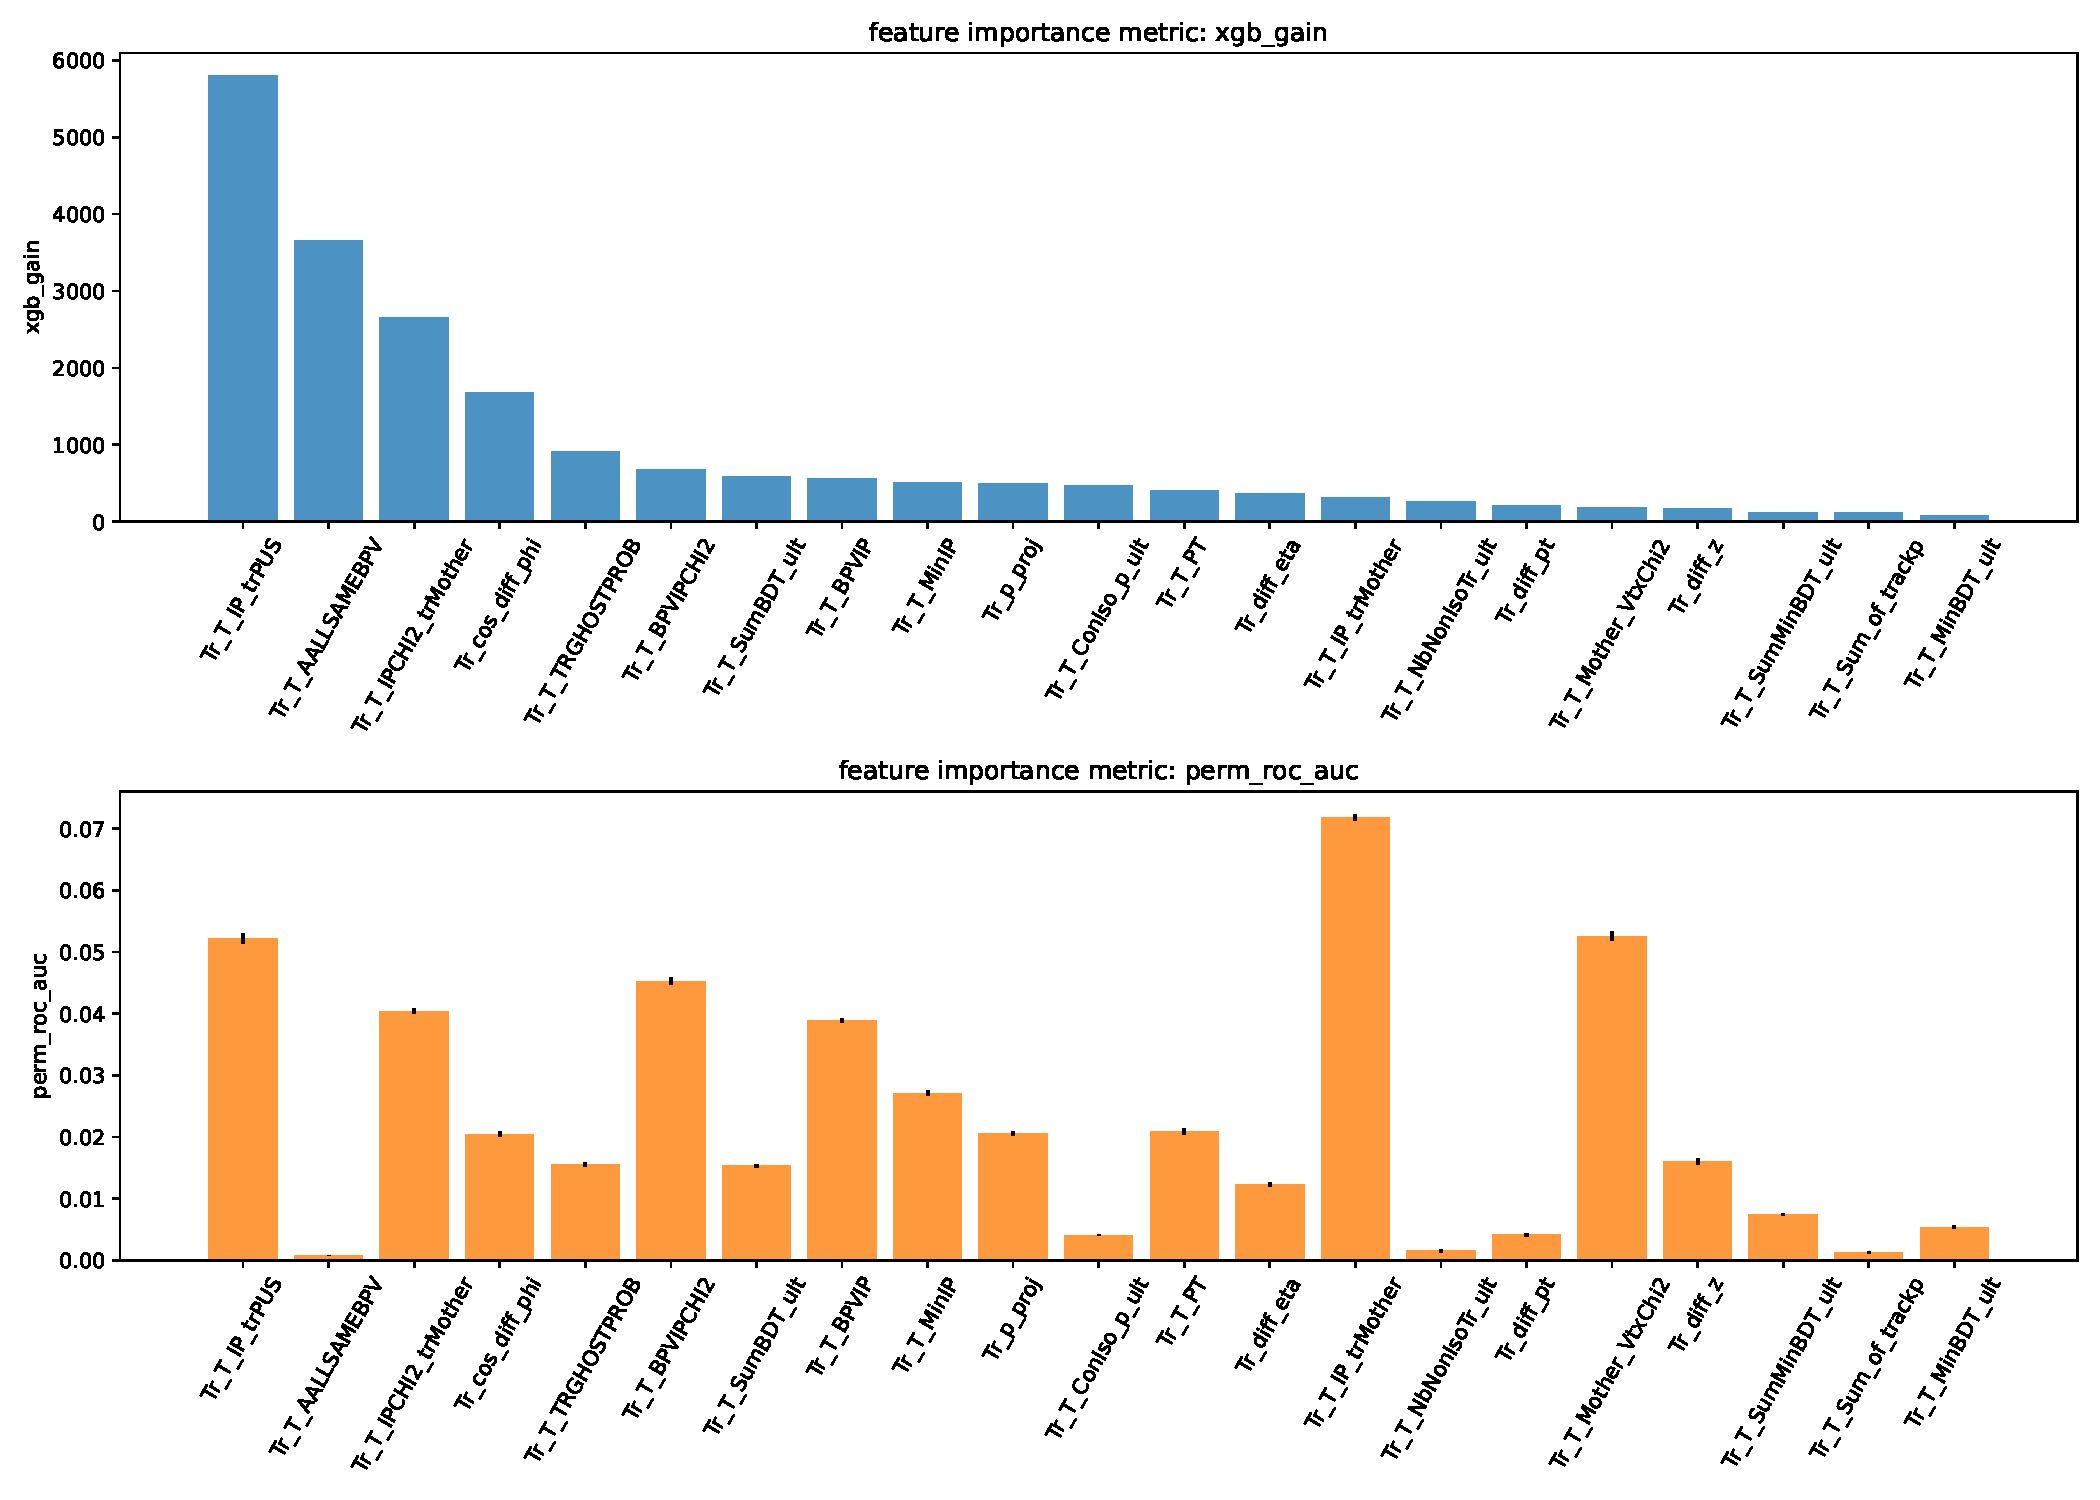
\includegraphics[width=\textwidth]{images/SS_feature_importances.pdf}
    \caption{Calculated feature importances on the trained DeepSet. Shown are the gains and the permutation importances of the ROC AUC normed on the largest value.}
    \label{fig:SS_importances}
\end{figure}

\begin{table}
    \centering
    \caption{List of all features used to train the BDT for SS track identification.}
    \label{tab:SS_features}
    \begin{tabular}{c c}
        \toprule
        feature & feature \\
        \midrule
        $p_\text{T}$        & $\text{IP}_\text{SV}$ \\ 
        $p_\text{proj}$     & $\chi^2(\text{IP}_\text{SV})$ \\ 
        $\Delta p_\text{T}$ & $\sigma(\text{IP}_\text{pileup vtx})$ \\ 
        $\Delta z$          & $\text{IP}_\text{best PV}$ \\    
        $\Delta \eta$       & $\chi^2(\text{IP}_\text{best PV})$ \\ 
        $\cos(\Delta \phi)$ & $\text{IP}_\text{min}$ \\ 
        $\text{Prob}_\text{ghost}$ & same PV \\
        $\chi^2(\text{vtx})$     & cone isolation \\
        SumBDT              & $N_\text{non iso}$ \\ 
        MinBDT              & $\sum p_\text{in cone}$ \\ 
        SumMinBDT           &  \\
        \bottomrule
    \end{tabular}
\end{table}

%(Explain all features)....
All the following features describe a single particle or rather its reconstructed track.
%
$p$ is the momentum and
$p_\text{T}$ is the transversal momentum. 
%
Between the signal $B$ and the particle,
$p_\text{proj}$ is the dot product of the 4-momenta,
$\Delta p_\text{T}$ is the difference of the transversal momenta,    
$\Delta \eta$ is the difference of the pseudorapidities and   
$\cos(\Delta \phi)$ is the cosine of the difference of the $\phi$-coordinates. 
$\Delta z$ is the $z$-coordinate difference of the PV and the first detector hit of the track. 
%  
$\text{Prob}_\text{ghost}$ is an estimated probability that the track is falsely reconstructed and does not belong to an actual particle. 
$\chi^2(\text{vtx})$ is the $\chi^2$ of the combined reconstructed vertex of the signal~$B$ and the track. 
\enquote{same PV} refers to whether the particle's vertex is the same as the PV.
%
An impact parameter (IP) is the minimum distance of a track to a given point.
$\text{IP}_\text{SV}$ is the IP to the SV and  
$\chi^2(\text{IP}_\text{SV})$ is its uncertainty.
$\sigma(\text{IP}_\text{pileup vtx})$ is the significance of the IP to the closest pileup vertex,
$\text{IP}_\text{best PV}$ is the IP to the best estimated PV and  
$\chi^2(\text{IP}_\text{best PV})$ is its uncertainty.
$\text{IP}_\text{min}$ is the minimum IP with respect to all PV candidates.
%
A cone-isolation refers to the existence of other tracks in a cone around the tagging track.
SumBDT,    
MinBDT and    
SumMinBDT describe the cone-isolation based on multiple BDT classifiers.
$\sum p_\text{in cone}$ is the sum of the absolute momenta of all particle tracks in cone-isolation cone.
The feature \enquote{cone isolation} describes the cone-isolation based $p/\sum p_\text{in cone}$. 
$N_\text{non iso}$ is the number of tracks not isolated from the tagging track.   

Then a BDT is trained on a dataset containing all features of this list.
From the $18$ million tracks in the dataset, $60\%$ are used for training and $40\%$ are used for validation of the trained model.
The trained model contains $2000$ estimators at a maximum decision tree depth of $4$.
The learning rate is set to $0.1$.
Due to the imbalance of SS tracks and other tracks in the data ($N_\text{other}/N_\text{SS} = 11.94$), a parameter that controls the balance of positive and negative weights of the BDT is set accordingly. 
The learning objective is logistic regression for binary classification.

The negative log-likelihood and the error rate for each iteration of the training of the BDT are shown in \cref{fig:SS_history}.
The error rate is the proportion of predictions matching the ground truth of the simulation.
For this, all tracks with $\text{Prob}_\text{SS}>0.5$ count as predicted SS tracks. 

\begin{figure}
    \centering
    \begin{subfigure}{0.5\textwidth}
        \centering
        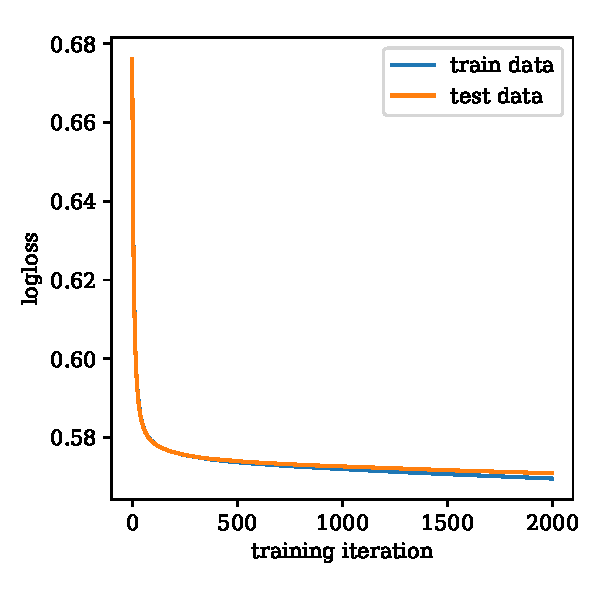
\includegraphics[width=\textwidth]{images/SS_history_logloss.pdf}
        \caption{negative log-likelihood}
    \end{subfigure}%
    \begin{subfigure}{0.5\textwidth}
        \centering
        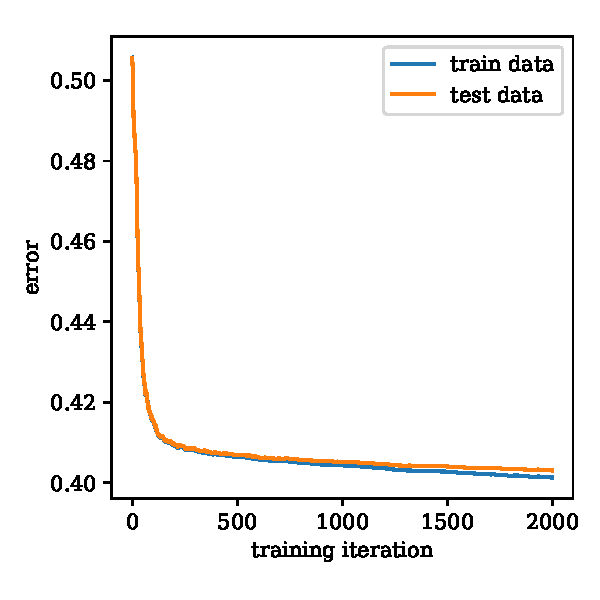
\includegraphics[width=\textwidth]{images/SS_history_error.pdf}
        \caption{error rate}
    \end{subfigure}%
    \caption{Training performance of the SS BDT.}
    \label{fig:SS_history}
\end{figure}

To show the achieved separation of the SS tracks, histograms of $\text{Prob}_\text{SS}$ split by the simulation ground truth are shown in \cref{fig:SS_output}.
A measure of separation is the ROC (reciever operating characteristic) curve shown in \cref{fig:SS_ROC}.
The achieved ROC AUC (area under the ROC curve) is $0.763$ on the test data and $0.767$ on the training data.
A ROC AUC of $1.0$ means perfect separation and a ROC AUC of $0.5$ means no separation.
To estimate the generalization and overtraining of the model, each performance measure is calculated on both the test data and training data.

\begin{figure}
    \centering
    \begin{subfigure}{0.5\textwidth}
        \centering
        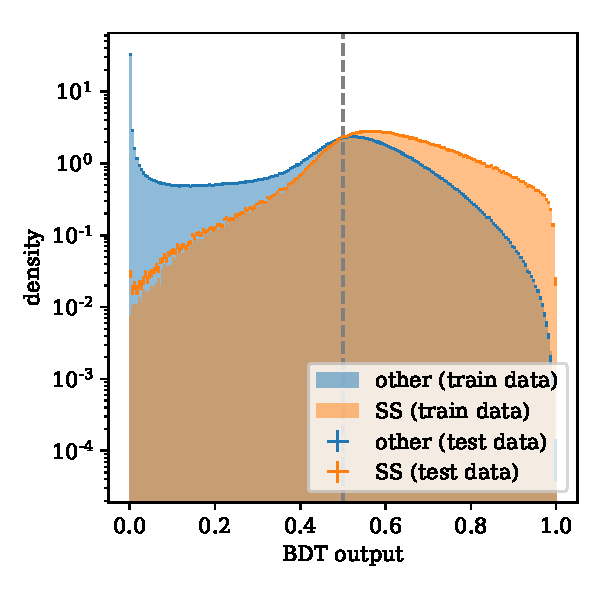
\includegraphics[width=\textwidth]{images/SS_output.pdf}
        \caption{distribution of $\text{Prob}_\text{SS}$}
        \label{fig:SS_output}
    \end{subfigure}%
    \begin{subfigure}{0.5\textwidth}
        \centering
        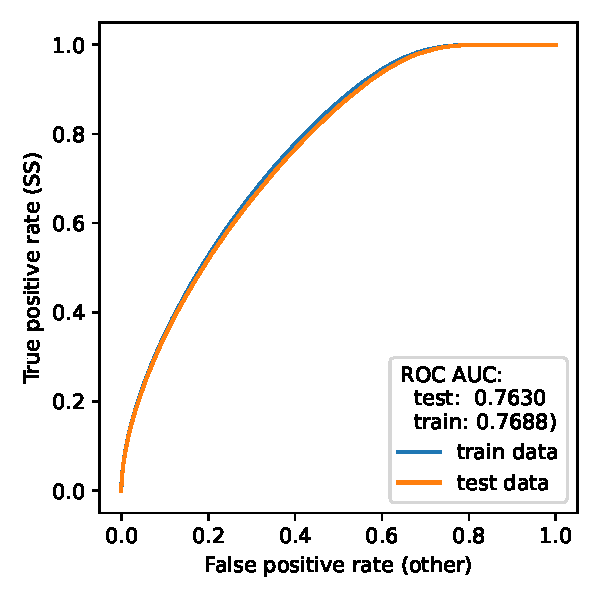
\includegraphics[width=\textwidth]{images/SS_ROC.pdf}
        \caption{ROC curve}
        \label{fig:SS_ROC}
    \end{subfigure}%
    \caption{The left figure shows the distribution of the BDT output split by the simulation ground truth. The right figure shows the ROC curve of the BDT output. Both figures show the BDT prediction for the test data and the training data.}
    \label{fig:SS_eval}
\end{figure}

\section[Classification of \texorpdfstring{$B_d$ and $B_s$}{Bd and Bs} mesons]{Classification of \texorpdfstring{$\symbf{B_d}$ and $\symbf{B_s}$}{Bd and Bs} mesons}

The distinction between $B_d$ and $B_s$ mesons based on the associated event is a non-trivial problem.
Since both mesons have different masses, it is expected that there is some difference in the kinematics of the associated event.
Therefore, it is tested if a multivariate machine learning algorithm can spot these differences.
The algorithm of choice for this thesis is a DeepSet that is trained on simulated LHCb data.
As explained in \cref{sec:DeepSet}, a DeepSet can handle data of variable length where the order of its elements should not change the result of the classification.
Therefore, DeepSets are ideal to classify $pp$-collision events that contain different amounts of particle tracks.
The DeepSet trained here, outputs an estimated probability $\text{Prob}_{B_s}$ for each event that the signal~$B$ is a $B_s$ meson.
Therefore, $1-\text{Prob}_{B_s}$ is the estimated probability that the signal~$B$ is a $B_d$ meson.
The implementation of the DeepSet is done with the library PyTorch \cite{pytorch}.

The procedure of selecting important features is similar to the procedure described in \cref{sec:SS_classifier}.
However, a DeepSet was trained on all features and the feature importances used here are the permutation importance of the ROC AUC and the permutation importance of the accuracy.
Again, features with the lowest feature importance scores are discarded until a reasonable amount of features is achieved.
The remaining 23 features are listed in \cref{tab:B_features} and the corresponding feature importances are shown in \cref{fig:B_importances}.

\begin{figure}
    \centering
    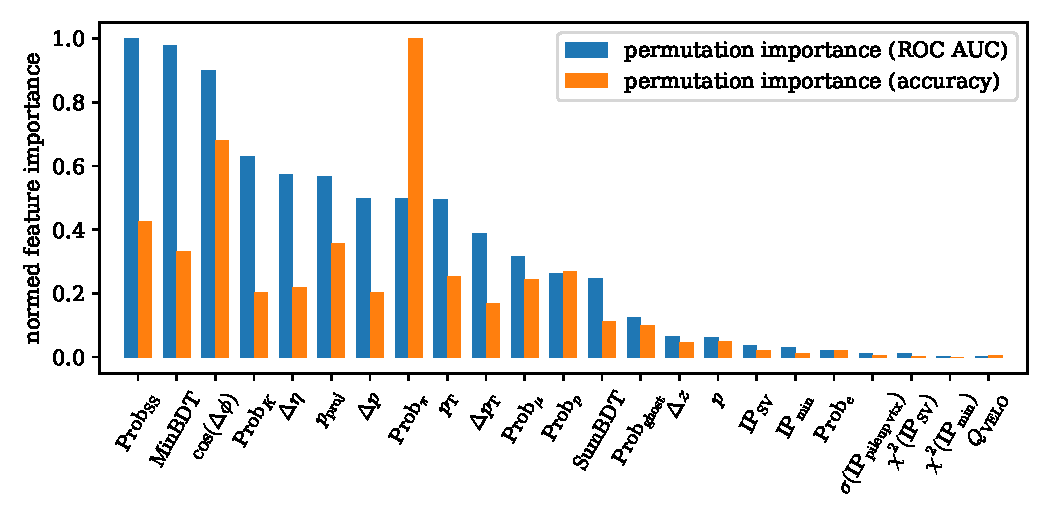
\includegraphics[width=\textwidth]{images/B_feature_importances.pdf}
    \caption{Calculated feature importances on the trained DeepSet. Shown are the permutation importances of the ROC AUC and the accuracy normed on the largest value.}
    \label{fig:B_importances}
\end{figure}

\begin{table}
    \centering
    \caption{List of all features used to train the DeepSet for B meson classification.}
    \label{tab:B_features}
    \begin{tabular}{c c}
        \toprule
        feature & feature \\
        \midrule
        $p$                 & $\text{Prob}_\text{SS}$ \\ %"Tr_T_P","Tr_ProbSS"
        $p_\text{T}$        & $\text{Prob}_e$ \\ %"Tr_T_PT", "Tr_T_PROBNNe"
        $p_\text{proj}$     & $\text{Prob}_\text{ghost}$ \\ %"Tr_p_proj","Tr_T_PROBNNghost"
        $\Delta p$          & $\text{Prob}_K$ \\ %"Tr_diff_p", "Tr_T_PROBNNk"
        $\Delta p_\text{T}$ & $\text{Prob}_\mu$ \\ %"Tr_diff_pt","Tr_T_PROBNNmu"
        $\Delta z$          & $\text{Prob}_p$ \\ %"Tr_diff_z", "Tr_T_PROBNNp"
        $\cos(\Delta \phi)$ & $\text{Prob}_\pi$ \\ %"Tr_cos_diff_phi", "Tr_T_PROBNNpi"
        $\Delta \eta$       & $\sigma(\text{IP}_\text{pileup vtx})$ \\ %"Tr_diff_eta", "Tr_T_IP_trPUS"
        $\text{IP}_\text{SV}$        & $Q_\text{VELO}$ \\ %"Tr_T_IP_trMother",  "Tr_T_VeloCharge"
        $\chi^2(\text{IP}_\text{SV})$    & SumBDT \\ %"Tr_T_IPCHI2_trMother", "Tr_T_SumBDT_ult"
        $\text{IP}_\text{min}$               & MinBDT \\ %"Tr_T_MinIP", "Tr_T_MinBDT_ult"
        $\chi^2(\text{IP}_\text{min})$           & \\ %"Tr_T_MinIPChi2"
        \bottomrule
    \end{tabular}
\end{table}

%(Explain all features)....
Multiple features that are used here are already described in \cref{sec:SS_classifier}.
These features are 
$p$,
$p_\text{T}$, 
$p_\text{proj}$, 
$\Delta p_\text{T}$, 
$\Delta z$, 
$\cos(\Delta \phi)$, 
$\Delta \eta$, 
$\text{Prob}_\text{ghost}$
$\text{IP}_\text{SV}$, 
$\chi^2(\text{IP}_\text{SV})$, 
$\text{IP}_\text{min}$,        
SumBDT and
MinBDT.
The other features used here are described in the following paragraph.

All the following features describe a single particle or rather its reconstructed track.
$\Delta p$ is the difference of the absolute momenta of the particle and the signal~$B$.
$\chi^2(\text{IP}_\text{min})$ is the uncertainty of $\text{IP}_\text{min}$.
%
$\text{Prob}_\text{SS}$ is an estimated probability that the track belongs to the SS and is the output of the classifier described in \cref{sec:SS_classifier}. 
$\text{Prob}_e$, 
$\text{Prob}_K$, 
$\text{Prob}_\mu$, 
$\text{Prob}_p$ and 
$\text{Prob}_\pi$ are estimated probabilities about the particle's type.
%
$Q_\text{VELO}$ is a measure for the interaction of the particle with the VELO detector based on the induced current due to material interactions and bremsstrahlung photons.


The final DeepSet trained here consists of a $\phi$-network that extracts 64 features about each track and a $\rho$-network with a single output.
The $\phi$-network has an input layer of size 23 followed by 3 layers with of sizes 64, 128 and 64.
The $\rho$-network has an input layer of size 64 followed by 3 layers of sizes 128, 64 and 1.
All hidden layers use the ReLU activation function and have a dropout rate of $50\%$.
The output layer of the $\rho$-network uses the sigmoid activation function.

From the $0.4$ million events in the dataset, $60\%$ are used for training and $40\%$ are used for validation of the trained model.
Before training or evaluation, each feature in the data is standardized using 
\begin{equation*}
    f(x) = \frac{x - \mu_i}{\sigma_i} \, .
\end{equation*} 
Where $\mu_i$ is the mean and $\sigma_i$ is the standard deviation of feature $i$ in the training data.

The DeepSet is trained using the loss function \enquote{binary cross entropy} and the optimizer \enquote{Adam}.
Using early stopping, the training is stopped at iteration 600 after 50 iterations without improvement on the validation dataset.
The loss and the error rate for each iteration of the training of the DeepSet are shown in \cref{fig:B_history}.

\begin{figure}
    \centering
    \begin{subfigure}{0.5\textwidth}
        \centering
        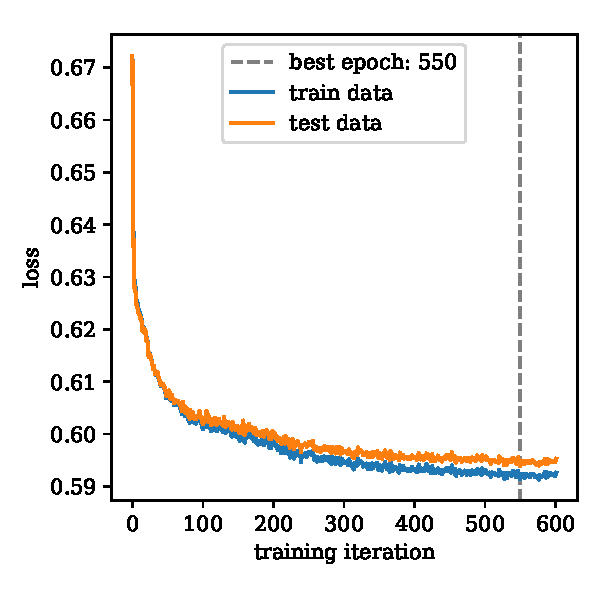
\includegraphics[width=\textwidth]{images/B_history_loss.pdf}
        \caption{binary cross entropy loss}
    \end{subfigure}%
    \begin{subfigure}{0.5\textwidth}
        \centering
        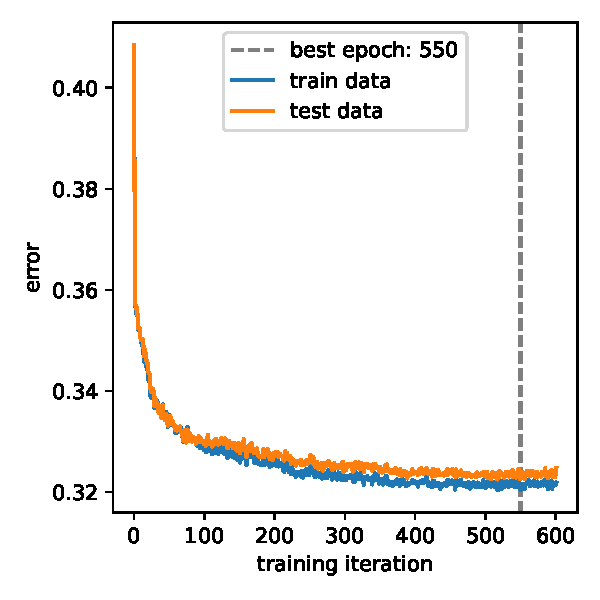
\includegraphics[width=\textwidth]{images/B_history_error.pdf}
        \caption{error rate}
    \end{subfigure}%
    \caption{Training performance of the DeepSet for $B$ meson classification.}
    \label{fig:B_history}
\end{figure}

To show the achieved separation of the $B$ mesons, histograms of $\text{Prob}_{B_s}$ split by the simulation ground truth are shown in \cref{fig:B_output}.
The achieved ROC curve is shown in \cref{fig:B_ROC} with a ROC AUC of $0.739$ on the test data and $0.742$ on the training data.
To estimate the generalization and overtraining of the model, each performance measure is calculated on both the test data and training data.

\begin{figure}
    \centering
    \begin{subfigure}{0.5\textwidth}
        \centering
        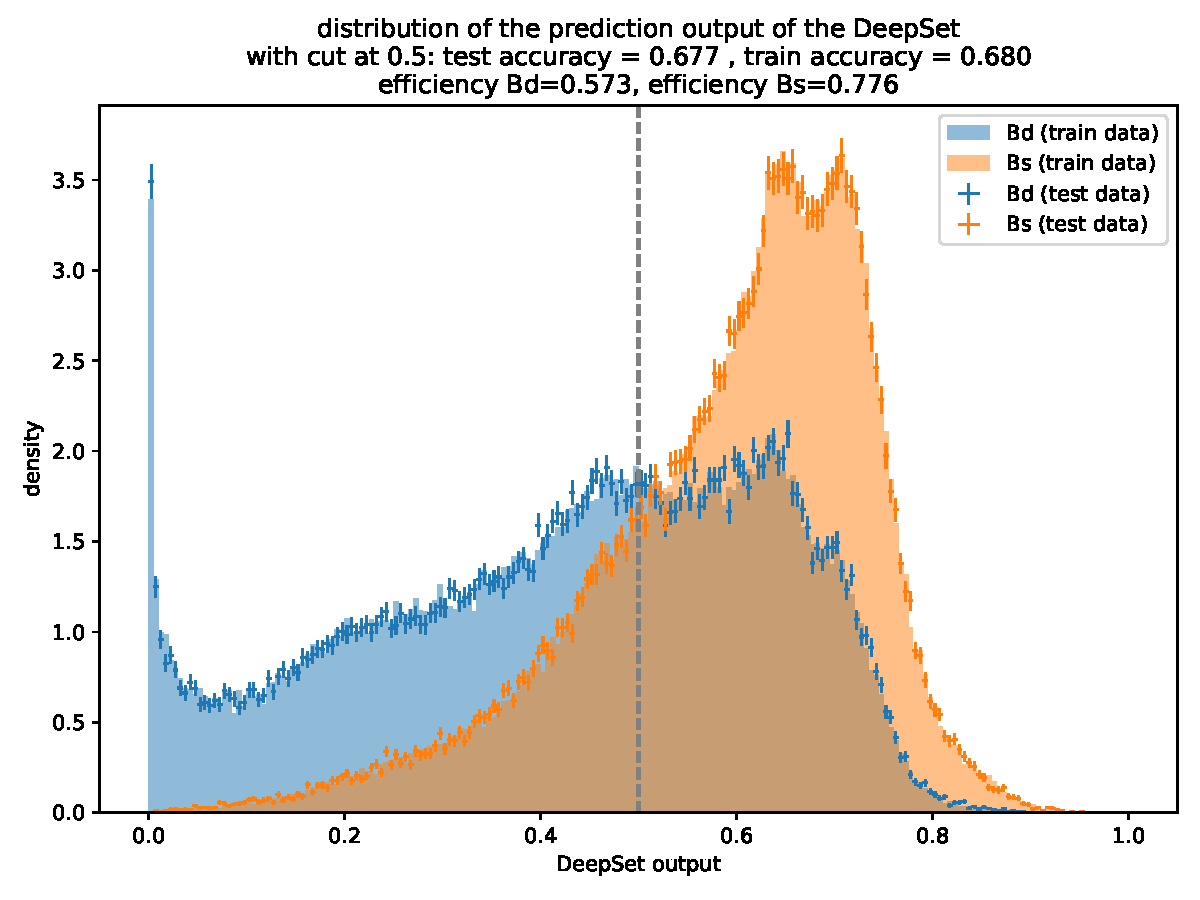
\includegraphics[width=\textwidth]{images/B_output.pdf}
        \caption{distribution of $\text{Prob}_{B_s}$}
        \label{fig:B_output}
    \end{subfigure}%
    \begin{subfigure}{0.5\textwidth}
        \centering
        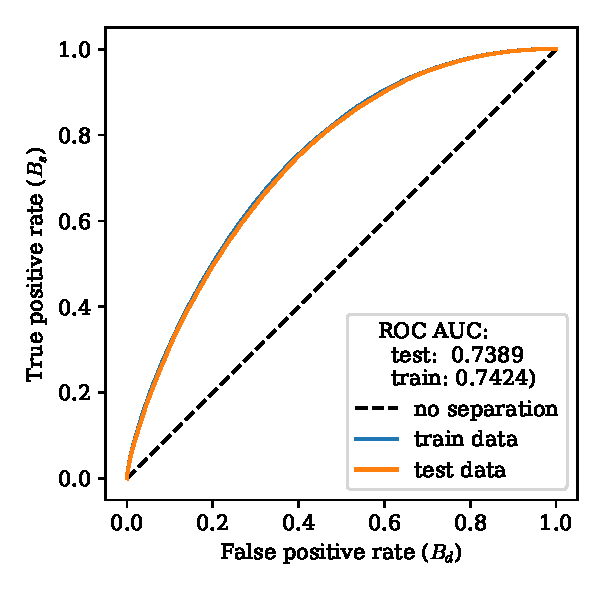
\includegraphics[width=\textwidth]{images/B_ROC.pdf}
        \caption{ROC curve}
        \label{fig:B_ROC}
    \end{subfigure}%
    \caption{The left figure shows the distribution of the DeepSet output split by the simulation ground truth. The right figure shows the ROC curve of the DeepSet output. Both figures show the DeepSet prediction for the test data and the training data.}
    \label{fig:B_eval}
\end{figure}

\section{Testing the algorithm on LHCb data}

%Training machine learning algorithms on simulated data assumes that the simulation contains the same patterns as found in real physics.%
%Training machine learning algorithms on simulated data assumes that the simulation is a good approximation of real world physics.
%Although the performance of trained models can be evaluated on data that was not used for training, 

%A necessary step in developing any algorithm is to check whether this algorithm works in scenarios that it is intended for.
%The trained model in this thesis is intended to distinguish $B_d$ from $B_s$ mesons in $pp$-collisions independent of the decay channel.
%Additionally, the model is intended to classify processes of the physical world rather than the simulations it is trained on.
%Consequently, the final step of this thesis is testing the model on LHCb run 2 data of the decay $B^0 \rightarrow J/\psi + K_\text{S}$.
%This decay channel contains both the $B_d$ and $B_s$ mesons and the data 

Although the developed model of this thesis is intended to distinguish $B_d$ from $B_s$ mesons in $pp$-collisions independent of the decay channel, it is trained only on simulated data containing the decay channels $B_d \rightarrow J/\psi \, K^*$ and $B_s \rightarrow D^+_s \, \pi^-$.
Consequently, the trained model must be evaluated on LHCb data of some other decay channel.
Chosen here are the decays $B_d \text{ or } B_s \rightarrow J/\psi \, K^0_\text{S}$.
The dataset used here contains LHCb data from the years 2016, 2017 and 2018 that has been selected for both mentioned decays using similar selection criteria. 

Since this dataset originates from a real measurement rather than a simulation, the data contains a significant amount of background events.
In order to be able to fit the $B_s$ resonance, the amount of background events is reduced.
The procedure used for background reduction is based on the work-in-progress measurement of $\sin(2\beta)$ in $B^0\rightarrow J/\psi \, K^0_\text{S}$ decays with run 2 data, and is explained here only very briefly.

A few types of background are reduced manually.
One source of such background events is the misidentification of $\Lambda^0 \rightarrow p^+ \, \pi^-$ decays as $K^0_\text{S} \rightarrow \pi^+ \, \pi^-$.
To reduce this type of background, events are rejected if the reconstructed invariant mass of the $K^0_\text{S}$~candidate is in the region  of the $\Lambda^0$~mass (\qtyrange{1095}{1140}{\MeV}) and $\text{Prob}_p > \num{0.10}$ is required. 
Misidentified backgrounds from $B \rightarrow J/\psi \, K^*$ decays are rejected by requiring that the kaon candidate has a lifetime longer than $\qty{0.5}{\pico\second}$.
Finally, a cut $\chi^2(\text{fit})<\num{5.0}$ is applied. %TODO: mention features before explanation %TODO: after the BDT

To reduce all other types of combinatorial background, a BDT is trained.
Again, the BDT is implemented in Python using the library XGBoost \cite{xgboost}.
For this, events of the mentioned dataset with a reconstructed signal~$B$ mass larger than $\qty{5450}{\MeV}$ are used as background events, and simulated events of the decay $B_d \rightarrow J/\psi \, K^0_\text{S}$ are used as signal events.
The BDT has a maximum tree depth of 2, is trained at a learning rate of $0.3$ and consists of 2000 estimators.
A ROC AUC score of $0.989$ is achieved on test data and the corresponding ROC curve is shown in \cref{fig:BKG_BDT_ROC}.
With this, events are classified as background events if the BDT output is smaller than $\num{0.5}$.

\begin{table}
    \centering
    \caption{List of all features used to train the BDT for the distinction between signal and background events.}
    \label{tab:BKG_BDT_features}
    \begin{tabular}{c c}
        \toprule
        feature & feature \\
        \midrule
        IP$(B^0)$                   & $p_\text{T}(\pi^+)$ \\% "B_IP_OWNPV","piplus_PT"
        IP$(J/\psi)$                & $p_\text{T}(\pi^-)$ \\% "Jpsi_IP_OWNPV","piminus_PT"
        IP$(K^0_\text{S})$          & $p_\text{T}(K^0_\text{S})$ \\% "KS0_IP_OWNPV","KS0_PT"
        IP$(\mu^+)$                 & $\eta(B^0)$ \\% "muplus_IP_OWNPV","B_LOKI_ETA"
        IP$(\mu^-)$                 & $\eta(K^0_\text{S})$ \\% "muminus_IP_OWNPV","KS0_LOKI_ETA"
        FD$(K^0_\text{S})$    & $p_z(K^0_\text{S})$ \\% "KS0_FD_OWNPV","KS0_PZ"
        $\chi^2(\text{fit})$  & \\% "B_LOKI_DTF_CHI2NDOF",
        \bottomrule
    \end{tabular}
\end{table}

The features used by the BDT are listed in \cref{tab:BKG_BDT_features} and describe the signal $B$ and its decay particles.
The symbols inside the brackets represent the corresponding particle in the signal decay.
IP$(x)$ is the impact parameter to the production vertex of particle $x$.
$p_\text{T}(x)$ is the transversal momentum of particle $x$.
$\eta(x)$ is the pseudorapidity of particle $x$.
$p_z(x)$ is the momentum of particle $x$ along the $z$-axis.
FD$(x)$ is the flight distance from the production vertex to the decay vertex of particle $x$.
Finally, $\chi^2(\text{fit})$ is the $\chi^2$ corresponding to the reconstruction of the entire signal decay.

\begin{figure}
    \centering
    \begin{subfigure}{0.5\textwidth}
        \centering
        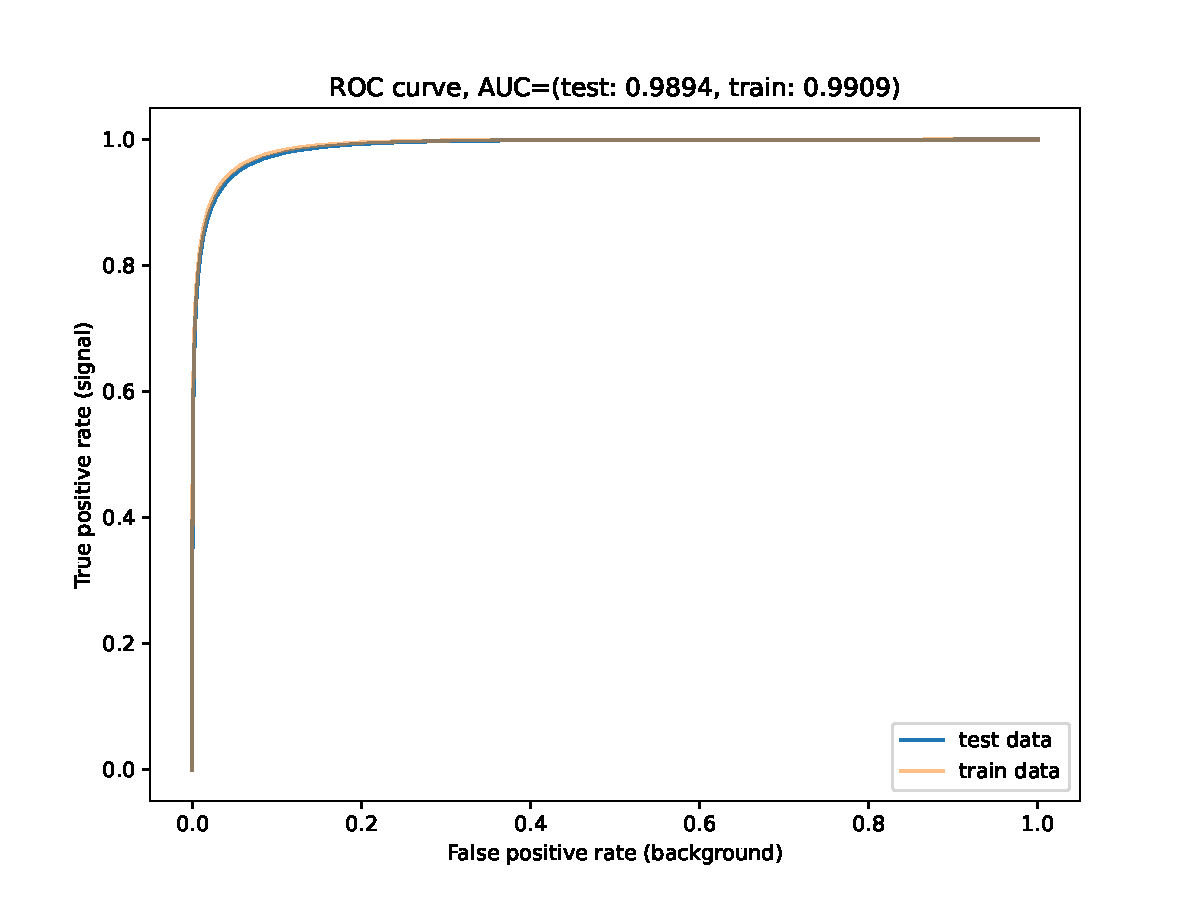
\includegraphics[width=\textwidth]{images/BKG_BDT_ROC.pdf}
        \caption{ROC curve of the BDT}
        \label{fig:BKG_BDT_ROC}
    \end{subfigure}%
    \begin{subfigure}{0.5\textwidth}
        \centering
        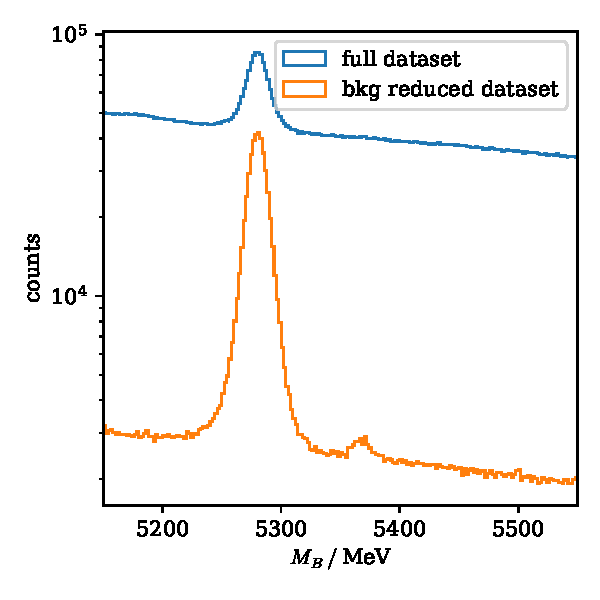
\includegraphics[width=\textwidth]{images/BKG_reduced.pdf}
        \caption{Distribution of the signal~$B$ mass}
        \label{fig:BKG_reduced}
    \end{subfigure}%
    \caption{The left figure shows the ROC curve achieved by the BDT for background identification. The right figure shows the distribution of the reconstructed signal~$B$ mass before and after reducing the background with the BDT and the manual cuts.}
    \label{fig:BKG_eval}
\end{figure}

\Cref{fig:BKG_reduced} shows the distribution of the reconstructed signal~$B$ mass before and after reducing the background with the BDT and the manual cuts.
After reducing the background, the trained model for the signal~$B$ classification is applied on the data to calculate $\text{Prob}_{B_s}$.
To estimate the performance of this prediction, an alternative method to estimate the amount of $B_d$ and $B_s$ mesons is needed.
The chosen procedure is to do a least squares fit on the $B$ mass distribution and estimate the counts of events by integrating each component of the fitted function.

In the following function definitions every variable except $M_B$ is a parameter that has to be fitted.
The $B$ mass distribution found in the data can be approximated by a function
\begin{equation}
    F(M_B) = N_\text{bkg} \cdot F_\text{bkg}(M_B) + N_{B_d} \cdot F_{B_d}(M_B) + N_{B_s} \cdot F_{B_s}(M_B)
\end{equation}
that is split into three components.
The first component $F_\text{bkg}$ describes the combinatorial background with 
\begin{align}
    F_\text{bkg}(M_B) = \exp(-\lambda \cdot M_B) \, .
\end{align}
The second component $F_{B_d}$ describes the events containing a $B_d$ meson and the third component $F_{B_s}$ describes the events containing a $B_s$ meson.
Both $F_{B_d}$ and $F_{B_s}$ use the same function
\begin{align} %TODO: only one equation number
    F_B(M_B) = &f_1 \cdot f_2 \cdot F_\text{CB}\left(\frac{M_B-\mu}{\sigma_1}, \beta_1, m_1\right) \\
                    &+ (1-f_1) \cdot f_2 \cdot F_\text{CB}\left(-\frac{M_B-\mu}{\sigma_2}, \beta_2, m_2\right) \\
                    &+ (1-f_1) \cdot (1-f_2) \cdot F_\text{gauss}\left(M_B,\mu,\sigma_3\right) \, ,
\end{align}
with the same parameters except $\mu_{B_s} = \mu_{B_d} + (M_{B_s}-M_{B_d})$.
$M_{B_d}=\qty{5279.65}{\MeV}$ is the mass of $B_d$ mesons and $M_{B_s}=\qty{5366.88}{\MeV}$ is the mass of $B_s$ mesons \cite{pdg}.
\begin{equation}
    F_\text{CB}(x,\beta,m) = 
     \begin{cases}
         N \cdot \exp(-\frac{x^2}{2}) & \text{for } x > -\beta \\
         N \cdot \left(\frac{m}{|\beta|}\right)^m \cdot \exp\left(-\frac{\beta^2}{2}\right) \cdot \left(\frac{m}{|b|}-|b| - x\right)^{-m} & \text{for } x \leq -\beta
     \end{cases}
\end{equation}
is called a Crystal Ball distribution and
\begin{equation}
    F_\text{gauss}\left(x,\mu,\sigma\right) = \frac{1}{\sqrt{2}\pi\sigma} \cdot \exp\left(-\frac{1}{2}\left(\frac{x-\mu}{\sigma}\right)^2\right)
\end{equation}
is called a normal distribution.

All the following fits are done using the library \enquote{iminuit}\cite{iminuit}.
First, a fit is done on the simulated data of the $B_d$ peak to fix the parameters $f_1,f_2,\beta_1,\beta_2,m_1$ and $m_2$ for all the following fits. 
This fit is shown in \cref{fig:fit_mc}.
Then, for 100 values of $x$ between 0 and 1, a selection with $\text{Prob}_{B_s} \leq x$ and a selection with $\text{Prob}_{B_s} \geq x$ is made.
A fit is done on each acquired $B$ mass distribution and the counts
\begin{align}
    n_{B_d} &= \int_{\qty{5170}{\MeV}}^{\qty{5450}{\MeV}} N_{B_d} \cdot F_{B_d}(M_B) \, \symup{d}M_B \:\:\text{ and} \\
    n_{B_s} &= \int_{\qty{5170}{\MeV}}^{\qty{5450}{\MeV}} N_{B_s} \cdot F_{B_s}(M_B) \, \symup{d}M_B
\end{align}
are calculated numerically.
One of those fitted distributions is shown in \cref{fig:fit_example}.

\begin{figure}
    \centering
    \begin{subfigure}{0.5\textwidth}
        \centering
        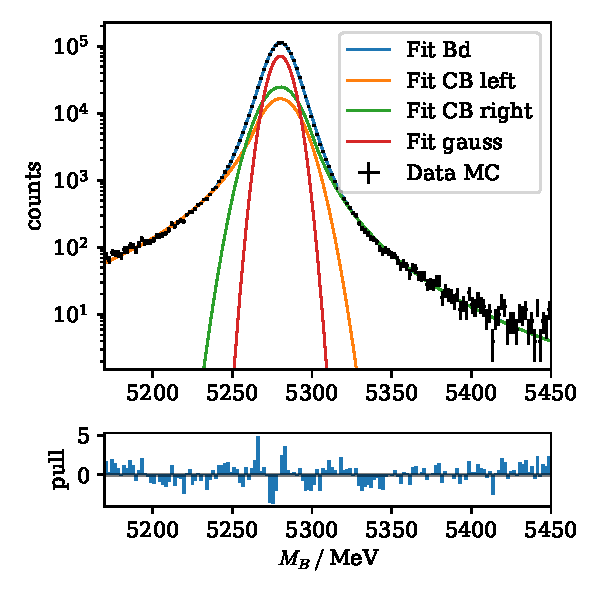
\includegraphics[width=\textwidth]{images/fit_mc.pdf}
        \caption{Fit of the $B_d$ peak}
        \label{fig:fit_mc}
    \end{subfigure}%
    \begin{subfigure}{0.5\textwidth}
        \centering
        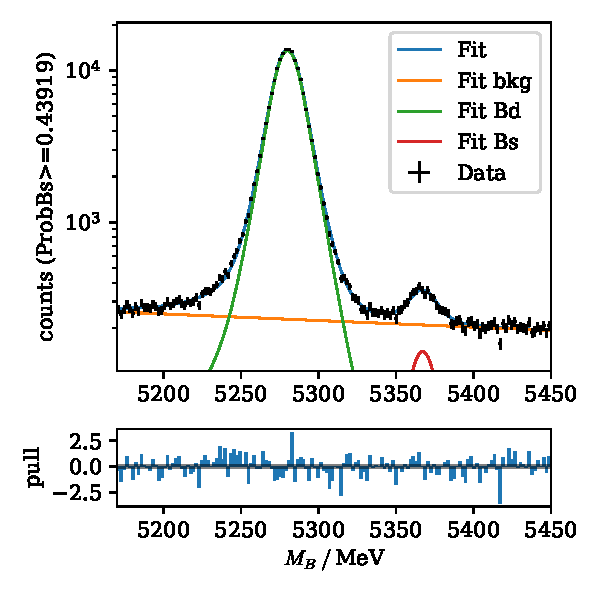
\includegraphics[width=\textwidth]{images/fit_example.pdf}
        \caption{Example fit of a data selection}
        \label{fig:fit_example}
    \end{subfigure}%
    \caption{The left figure shows a fit on simulated data of the $B_d$ peak. The right figure shows a fit of the $B$ mass distribution with the selection $\text{Prob}_{B_s} \geq 0.43919$. Both figures also show a pull distribution between the data points and the fit.}
\end{figure}

To estimate how good the trained model of this thesis can distinguish $B_d$ and $B_s$ mesons, the ratio $n_{B_s}/n_{B_d}$ is plotted by the cut value $x$ for selections with $\text{Prob}_{B_s} \geq x$. 
This is shown in \cref{fig:data_ratio}.
The expected value without any achieved separation is 
\begin{equation}
    \frac{\text{BR}(B_s \rightarrow J/\psi \, K^0_\text{S})}{\text{BR}(B_d \rightarrow J/\psi \, K^0_\text{S})} \cdot 
    f_s/f_d(\qty{13}{\TeV}) = \num{0.0109\pm0.0010} \, .
\end{equation}
Where the branching ratios are $\text{BR}(B_s \rightarrow J/\psi \, K^0_\text{S}) = \num{4.37\pm0.16e-4}$ and $\text{BR}(B_d \rightarrow J/\psi \, K^0_\text{S}) = \num{1.88\pm0.15e-5}$ \cite{pdg}, and $f_s/f_d(\qty{13}{\TeV}) = \num{0.2539\pm0.0079}$ is the ratio of the $B^0_s$ and $B^0$ fragmentation fractions in $pp$-collisions at $\qty{13}{\TeV}$ collision energy \cite{fsfd}.

Another approach to show the achieved separation, is to plot a curve similar to a ROC curve. 
For each selection, the estimated efficiencies
\begin{equation}
    \varepsilon_{B_d} = \frac{n_{B_d}(x)}{n_{B_d}(\text{no cut})} \quad\text{ and }\quad \varepsilon_{B_s} = \frac{n_{B_s}(x)}{n_{B_s}(\text{no cut})}
\end{equation}
are calculated. Shown in \cref{fig:data_roc} is the plot of $\varepsilon_{B_d}$ against $\varepsilon_{B_s}$.
Similar to a ROC curve, a diagonal line from $(0,0)$ to $(1,1)$ is the expectation without any achieved separation.
Compared to the achieved ROC curve on the simulated data shown in \cref{fig:B_ROC}, a substantially weaker separation is achieved on the LHCb data.

\begin{figure}
    \centering
    \begin{subfigure}{0.5\textwidth}
        \centering
        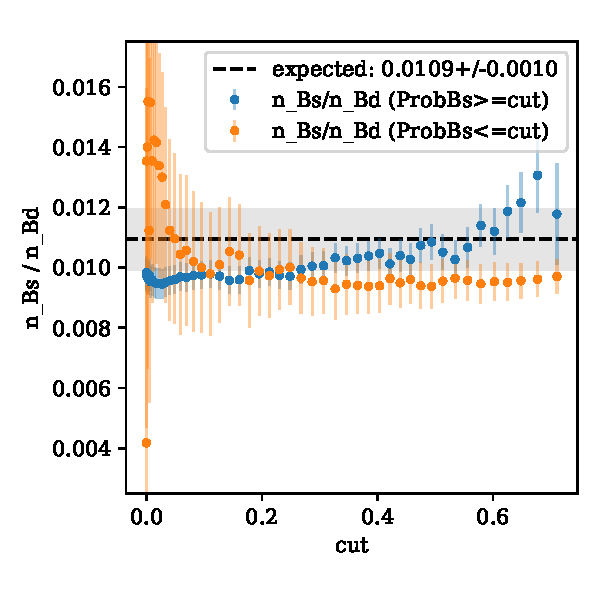
\includegraphics[width=\textwidth]{images/data_ratio.pdf}
        \caption{Ratio $n_{B_s}/n_{B_d}$ by cut value}
        \label{fig:data_ratio}
    \end{subfigure}%
    \begin{subfigure}{0.5\textwidth}
        \centering
        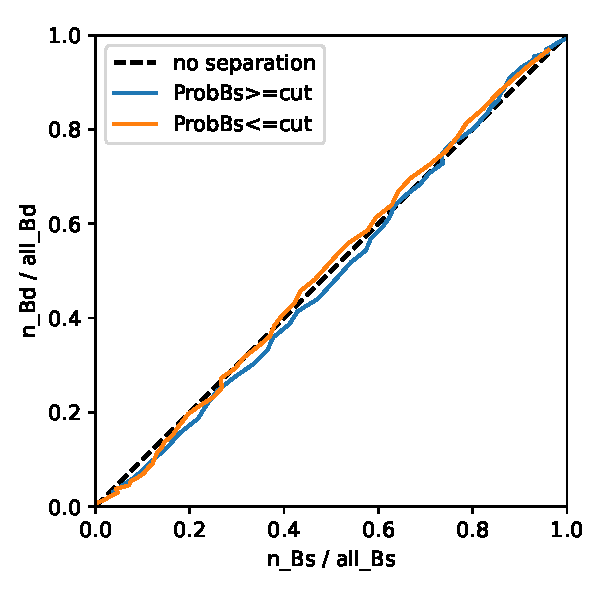
\includegraphics[width=\textwidth]{images/data_roc.pdf}
        \caption{similar to a ROC curve}
        \label{fig:data_roc}
    \end{subfigure}%
    \caption{The left figure shows the estimated ratio $n_{B_s}/n_{B_d}$. Here, it is important to note that selections with $\text{Prob}_{B_s} \leq x$ on small $x$ have a very small $B_s$ peak, which makes the interpretation of these ratios almost impossible. The right figure shows the estimated efficiencies $\varepsilon_{B_d}$ agains $\varepsilon_{B_s}$. In both figures, selections with $\text{Prob}_{B_s} \geq x$ are shown in blue and selections with $\text{Prob}_{B_s} \leq x$ are shown in orange.}
\end{figure}


